\vspace{5em}
\section{\huge Formalismo della MQ ad un determinato istante di tempo}

L'obiettivo di questo capitolo \'e introdurre un formalismo generale che possa essere applicato a una vasta classe di sistemi per la descrizione degli stati e delle grandezze fisiche osservabili delle quali vogliamo saper calcolare i risultati della misura, la probabilit\'a che una loro misura fornisca un determinato valore e, a partire da questo, il valore medio in uno stato e la fluttuazione attorno un valore arbitrario. Tutto questo deve essere fatto in accordo con le caratteristiche fondamentali della MQ: l'interpretazione probabilistica, le relazioni di indeterminazione e la quantizzazione di certe grandezze fisiche.

Iniziamo imponendo alcune restrizioni semplificartici:
\begin{enumerate}
\item Consideriamo sistemi con un numero finito N di gradi di libert\'a 

\item Daremo una trattazione non relativistica della MQ, che ci permetter\'a di considerare in modo diverso lo spazio-tempo, non pi'u come semplici coordinate, ma come operatori. Questi limiti saranno superati poi con la teoria relativistica dei campi.

\item adotteremo un formalismo hamiltoniano per la descrizione del sistema fisico
\end{enumerate}

\subsection{Descrizione degli stati}

Conoscere lo stato di un sistema fisico significa avere a disposizione l'informazione massima che possiamo acquisire su tale sistema effettuando operazioni che siamo fisicamente in grado di eseguire su di esso (\textit{stato puro}), ma anche un'informazione parziale se per qualche motivo quella massima ci 'e preclusa (\textit{stati misti}), a cui poi dovremmo applicare i concetti della fisica statistica.


\subsubsection{Stati in MC}

In MC la descrizione dello stato di un sistema 'e completamente determinata nel momento in cui abbiamo a disposizione i valori delle coordinate generalizzate e dei loro momenti coniugati, misurati ad un tempo iniziale $t_0$:

$$[q_i(t_0), p_i(t_0)]_{i=1, \ldots, N}$$

Sappiamo dal formalismo hamiltoniano classico che, note queste condizioni iniziali, lo stato del sistema a qualsiasi istante successivo $t > t_0$ \'e completamente determinato attraverso le equazioni del moto

\begin{equation}
	{\dot{q}}_{i}={\frac{\partial H}{\partial p_{i}}}\qquad\qquad{\dot{p}}_{i}=-{\frac{\partial H}{\partial q_{i}}}
\end{equation}

Conoscendo con precisione arbitraria le condizioni iniziali, possiamo conoscere ugualmente con precisione arbitraria anche le $[q_i(t), p_i(t)]$ per istanti successivi e le funzioni $f(q, p)$ di queste due osservabili, grazie all'introduzione delle parentesi di Poisson:

$${\frac{\mathrm{d}f}{\mathrm{d}t}}=\sum_{i=1}^{N}{\frac{\partial f}{\partial q_{i}}}{\frac{\mathrm{d}q_{i}}{\mathrm{d}t}}+{\frac{\partial f}{\partial p_{i}}}{\frac{\mathrm{d}p_{i}}{\mathrm{d}t}}=\sum_{i=1}^{N}{\frac{\partial f}{\partial q_{i}}}{\frac{\partial H}{\partial p_{i}}}-{\frac{\partial f}{\partial p_{i}}}{\frac{\partial H}{\partial q_{i}}}=\{f,H\}$$


\subsubsection{Stati In MQ}

Dal punto di vista quantistico questa trattazione non \'e accettabile perch\'e viola il principio di indeterminazione, che non ci consente di conoscere simultaneamente i valori delle variabili tra loro coniugate con precisione arbitraria, ma anche perch\'e dobbiamo considerare l'aspetto probabilistico della MQ.

Per capire come generalizzare la descrizione dell'evoluzione dello stato in MQ consideriamo un sistema molto semplice di una singola particella priva di spin, che si muove in una dimensione spaziale infinita $x$. Lo stato di questa particella \'e descritto dalla funzione d'onda $\Psi(x)$, che ovviamente non potr\'a essere una funzione qualsiasi, ma dovr\'a rispettare alcune regole fondamentali per poter essere associata alla particella. Dal contributo di Born, sappiamo che $\Psi(x)$ \'e legata alla densit\'a di probabilit\'a $P(x)$ di trovare la particella in un intorno della posizione $x$, per cui dovr\'a necessariamente essere:

\begin{equation}
	P(x)\geq0 \qquad \int{\rm d}x\,P(x)=1\qquad P(x)=\frac{|\Psi(x)|^{2}}{\parallel\Psi(x)\parallel^{2}}
\end{equation}

Da questa definizione ricaviamo due condizioni a cui deve sottostare la funzione d'onda: innanzitutto non pu\'o essere una funzione identicamente nulla, matematicamente perch\'e avrebbe norma nulla e quindi la frazione divergerebbe, fisicamente perch\'e non descriverebbe alcuno stato, in secondo luogo dovr\'a appartenerne a quel gruppo di funzioni modulo quadro integrabili per poter rispettare la condizione imposta dalla probabilit\'a, chiamiamo questo gruppo $L_2(\mathbb{R})$

\begin{equation}
	\left\|\Psi\right\|^{2}=\int{\rm d}x\left|\Psi\right|^{2}<\infty\quad\text{e} \quad\Psi(-\infty)=\Psi(+\infty)=0\quad\longrightarrow\quad\Psi(x)\in L_{2}(\mathbb{R})
\end{equation}

Osserviamo che se $\Psi(x)$ descrive lo stato di un sistema, anche $\alpha\Psi(x)$ con $\alpha \in \mathbb{C} - {0}$ descrive lo stesso stato, perch\'e nel calcolo della densit\'a di probabilit\'a la costante moltiplicativa si elide e otteniamo lo stesso risultato.


\textbf{Richiami sugli spazi di Hilbert}

Dato che $L_2(\mathbb{R})$ \'e uno \textit{spazio di Hilbert}, richiamiamo alcuni concetti fondamentali su questi spazi. $\mathcal{H}$ \'e uno \textit{spazio vettoriale complesso}, i cui vettori si indicano con il simbolo di \textit{ket} $|\Psi\rangle$; questo significa che presi due vettori in esso, anche la loro combinazione lineare appartiene a $\mathcal{H}$

$$\alpha,\beta\in\mathbb{C}\quad \text{e}\quad(|\Psi\rangle\,,|\Phi\rangle)\in\mathcal{H}\quad\longrightarrow\quad(\alpha\,|\Psi\rangle+\beta\,|\Phi\rangle\,)\in\mathcal{H}\,$$
ci'o 'e necessario per la linearit\'a della MQ che fa valere il principio di sovrapposizione. Poi, 'e presente un *prodotto* scalare definito positivo, cio'e possiamo associare a due vettori uno specifico numero complesso

$$(\left|\Psi\right\rangle,\left|\Phi\right\rangle)\in{\mathcal{H}}\quad\longrightarrow\quad\left\langle\Psi|\Phi\right\rangle\in{\mathbb{C}}$$

che gode delle ben note propriet\'a:

$$\langle\Psi|\Phi\rangle=\langle\Phi|\Psi\rangle^{*}$$
$$\braket{\Phi}{\lambda_{1}\Psi_1 + \lambda_{2}\Psi_2} = \lambda_{1}\braket{\Phi}{\Psi_{1}} + \lambda_{2}\braket{\Phi}{\Psi_{2}} \qquad\qquad 
\braket{\lambda_{1}\Psi_{1} + \lambda_{2}\Psi_{2}}{\Phi} = \lambda_{1}^* \braket{\Psi_{1}}{\Phi} + \lambda_{2}^* \braket{\Psi_{2}}{\Phi}$$
$$||\Psi||2 = \braket{\Psi}{\Psi} \geq 0 \qquad\qquad = 0 \iff \ket{\Psi} = 0$$

Inoltre $\mathcal{H}$ \'e \textit{completo}, cio\'e ogni successione di Cauchy $\{\ket{\Psi_n}\}$ converge in $\mathcal{H}$:

$$\operatorname*{lim}_{m,n\to\infty}||\Psi_{m}-\Psi_{n}||=0\quad\exists\,|\Psi\rangle\in{\mathcal{H}}\quad\left|\quad\operatorname*{lim}_{n\to\infty}||\Psi-\Psi_{n}||=0\right.$$

Infine \'e \textit{separabile}, quindi esistite una base numerabile e densa ovunque per i vettori di $\mathcal{H}$, e non \'e restrittivo prenderla ortonormale $\{\ket{u_n}\}$. Questo ci consente di scrivere ogni vettore dello spazio di Hilbert come combinazione lineare dei vettori di base

$$|\Psi\rangle=\sum_{n}c_{n}\,|u_{n}\rangle\qquad\langle u_{n}|u_{m}\rangle=\delta_{m n}$$

e moltiplicando a destra per il \textit{bra} $\bra{u_n}$ (un \textit{bra} altro non \'e che il complesso coniugato di un vettore) otteniamo la relazione

$$\langle u_{n}|\Psi\rangle=c_{n}\quad\longrightarrow\quad|\Psi\rangle=\sum_{n}|u_{n}\rangle\,\langle u_{n}|\Psi\rangle$$

Ci\'o che abbiamo fatto ha un importante risvolto pratico che scopriremo proseguendo nello studio della MQ,
infatti la quantit\'a $\sum_n \ket{u_n}\bra{u_n}$ rappresenta l'operatore identit\'a e si chiama \textit{relazione di completezza} dello spazio hilbertiano, si usa spessissimo nell'ambito degli operatori.

Notiamo che se prendiamo un'arbitraria combinazione lineare dei vettori di base dello spazio di Hilbert, infinita e numerabile, non \'e detto che il vettore corrispondente sia in $L_2$, perch\'e \'e necessario verificare che abbia norma finita, cio\'e che i suoi coefficienti soddisfino

$$\langle\Psi|\Psi\rangle=\sum_{n}|c_{n}|^{2}<\infty$$

Tutta l'informazione fornita da $\Psi(x)$ \'e reperibile anche dalla sua trasformata di Fourier, 

${\tilde{\Psi}}(p)=\left[L_{2}(\mathbb{R})\right]_{p}$

$$\tilde{\Psi}(p) = \frac{1}{\sqrt{2\pi\hbar}} \int \mathrm{d}x \Psi(x) e^{-i\frac{px}{\hbar}} \qquad\qquad \text{con} \Psi(x) = \frac{1}{\sqrt{2\pi\hbar}} \int \mathrm{d}p \tilde{\Psi} e^{i\frac{px}{\hbar}} \text{ antitrasformata}$$

il cui spazio di appartenenza \'e isomorfo $L_2(\mathbb{R})$. La presenza di $\hbar$ come fattore di normalizzazione e come fattore dell'esponenziale \'e dovuto al fatto che nella definizione rigorosa \'e presente il vettore d'onda $k$, legato al momento dalla relazione $k = \frac{p}{\hbar}$. La trasformata \'e una funzione definita nello spazio delle $p$ da cui \'e possibile ricavare la densit\'a di probabilit\'a di trovare una particella in un intorno di un determinato valore dell'impulso, in modo analogo a quanto fatto per la funzione nello spazio delle coordinate

$$P(p)=\frac{|\tilde{\Psi}(p)|^{2}}{||\tilde{\Psi}(p)||^{2}}$$

Tra trasformata e antitrasformata vale l'\textit{identit\'a di Parseval}, per la quale descrivere il sistema in un modo o nell'altro \'e del tutto equivalente 

$$||\Psi||^2 = ||\tilde{\Psi}||^2$$

Quanto appena detto deriva dal fatto che possiamo dimostrare che tutti gli spazi di Hilbert che hanno la stessa cardinalit\'a sono isomorfi tra loro; questo fatto ci suggerisce di sviluppare un formalismo in cui lo stato del sistema non sia legato alla particolare scelta della variabile da cui dipende la funzione d'onda, ma che ci sia un \textit{vettore astratto} di uno spazio di Hilbert, poi se risulta necessario potremo specificare una \textit{rappresentazione concreta}.

Detto questo, enunciamo il primo postulato della MQ:

\textbf{\textit{Postulato 1. Degli stati}} 

\textit{Ogni sistema quantistico $\mathcal{S}$ pu\'o essere associato ad uno spazio di Hilbert astratto $\mathcal{H}$, e ogni stato (puro) $\Sigma$ del sistema pu\'o essere associato a un raggio vettore complesso $\hat{\Psi} \in \mathcal{H}$.}

Introduciamo quindi la nozione importante di \textit{raggio vettore}, che \'e definito come la classe di equivalenza dei vettori che puntano nella stessa direzione

$${\hat{\Psi}}=\{\lambda\,|\Psi\rangle\quad\big|\quad\lambda\in\mathbb{C}-0\}$$

infatti come abbiamo detto in precedenza, tutti i $\lambda \ket{Psi}$ rappresentano lo stesso stato. Per rappresentare un raggio vettore possiamo scegliere un qualsiasi elemento rappresentativo della classe, solamente per comodit\'a lo prendiamo normalizzato, nel caso non lo fosse non dobbiamo dimenticare il fattore di normalizzazione necessario nella definizione di probabilit\'a.

Notiamo alcune cose: la prima \'e che la presenza della costante $\lambda$ include la possibilit\'a di avere una fase arbitraria pur essendo presente la normalizzazione, la seconda \'e che nel postulato valgono le implicazioni opposte, cio\'e a uno spazio di Hilbert \'e associabile un sistema quantistico e ad una raggio vettore uno stato puro, tranne in alcuni casi particolari che non tratteremo.


\textbf{Rappresentazioni $x$ e $p$}

Quando in MC abbiamo parlato di onde, abbiamo detto che quelle piane monocromatiche, che sono infinitamente estese, non sono realizzabili fisicamente ma le abbiamo comunque sfruttate per determinare la struttura matematica dei pacchetti, che invece hanno estensione ed energia finite, mediante integrale di Fourier.

Ora siamo di fronte allo stesso tipo di problema e la soluzione finale avr\'a la stessa struttura logica: abbiamo scritto $\Psi(x)$ come l'integrale di Fourier di esponenziali pesati da opportuni coefficienti dati dalla trasformata:

$$u_{p}(x)={\frac{1}{\sqrt{2\pi\hbar}}}e^{i{\frac{p x}{\hbar}}}\ \ \ \ \notin L_{2}(\mathbb{R})$$

Notiamo subito che questo tipo di funzioni non sono modulo quadro integrabili, tuttavia ci\'o non ci impedisce di interpretare questo insieme di oggetti come una \textit{base ortonormale generalizzata nel senso delle distribuzioni}, per le quali vale la relazione di ortonormalit\'a generalizzata (con la $\delta$ di Dirac) e di completezza

$$u_{p}u_{p}^{\prime}=\int\mathrm{d}x\,u_{p}^{*}(x)u_{p^{\prime}}(x)=\frac{1}{2\pi}\int\frac{d x}{\hbar}e^{-i\,\frac{x}{\hbar}(p-p^{\prime})}=\delta(p-p^{\prime})$$

$$\int\mathrm{d}x\,u_{p}^{*}(x^{\prime})u_{p}(x)=\frac{1}{2\pi}\int\frac{d x}{\hbar}e^{-i\frac{p}{\hbar}(x-x^{\prime})}d x=\delta(x-x^{\prime})$$

Allo stesso modo possiamo introdurre una base generalizzata con indici continui legati alla posizione della particella: $\xi_{x_0} (x) = \delta(x - x_0) \notin L_2(\mathbb{R})$

$$(\xi_{x_{0}},\xi_{x_{0}^{\prime}})=\int\mathrm{d}x\,\delta(x-x_{0})\delta(x-x_{0}^{\prime})=\delta(x_{0}-x_{0}^{\prime})$$
$$\int\mathrm{d}x_{0}\,\xi_{x_{0}}^{*}(x^{\prime})\xi_{x_{0}}(x)=\int\mathrm{d}x_{0}\,\delta(x_{0}-x^{\prime})\delta(x_{0}-x)=\delta(x-x^{\prime})$$  

A queste basi possiamo associare i \textit{ket} generalizzati $|x_{0}\rangle\,,|p_{0}\rangle$ e scrivere le relazioni di completezza generalizzate 

$$\begin{matrix}\langle x_0|x'_0\rangle=\delta(x_0-x'_0)&\int\mathrm{d}x_0\,|x_0\rangle\langle x_0|=1\\ \langle p_0|p_0\rangle=\delta(p_0-p_0')&\int\mathrm{d}p_0\,|p_0\rangle\langle p_0|=1\end{matrix}$$ 

grazie alle qual possiamo scrivere la funzione d'onda in modo estremamente intuitivo ed efficace
 
$$\langle x|\Psi\rangle=\langle x|\mathbbm{1}|\Psi\rangle=\int\mathrm{d}x\,\langle x|x_{0}\rangle\,\langle x_{0}|\Psi\rangle=\delta(x-x_{0})\int\mathrm{d}x^{\prime}\,\xi_{x_{0}}^{*}(x^{\prime})\Psi(x^{\prime})=\int\mathrm{d}x^{\prime}\,\delta(x-x^{\prime})\Psi(x^{\prime})=\Psi(x)\,.$$
$$\langle p|\Psi\rangle=\ldots={\tilde{\Psi}}(p)$$

\subsection{Descrizione delle osservabili}

Le osservabili sono tutte quelle quantit\'a che possiamo misurare con operazioni fisicamente eseguibili sul sistema, come per esempio l'energia, la velocit\'a, la posizione, ecc. Tutto ci\'o che possiamo sperare di misurare in laboratorio sulle osservabili \'e il valore medio in un dato stato.

\subsubsection{Spettro di un'osservabile}

In generale dobbiamo distinguere tra l'osservabile fisica e l'operatore matematico che la descrive, quindi chiamiamo A la prima e A il secondo. Possiamo per\'o identificare i due oggetti in base al postulato 3 che enunceremo in seguito, quindi la maggior parte delle volte verr\'a meno la distinzione tra i due.

Misurando questa osservabile, otteniamo certi valori che racchiudiamo in un insieme chiamato \textit{spettro}:

\textbf{Definizione 1.} \textit{Lo spettro di un'osservabile, che scriviamo come $\sigma(\mathcal{A})$, \'e l'insieme dei valori che possiamo ottenere con una misura di $\mathcal{A}$ prendendo in considerazione tutti i possibili stati del sistema}.

Ovviamente si deve verificare che $\sigma \mathcal{A} \subseteq \mathbb{R}$ dato che stiamo parlando di misure fisicamente eseguibili (di certo non potremmo trovare un valore complesso). Lo spettro di un'osservabile pu\'o essere sia \textit{puramente discreto} (come per esempio quello per una particella senza spin in una buca di potenziale infinita), oppure \textit{puramente continuo} (per una particella libera); in alcune occasioni pu\'o presentarsi uno \textit{spettro misto} dato dalla somma di una parte discreta e di una continua (\'e il caso della particella in una buca di potenziale di profondit\'a finita),
quindi in generale scriviamo 

$$\sigma(\mathcal{A}) = \sigma_d(\mathcal{A}) + \sigma_{c}(\mathcal{A})$$

Vediamo ora cosa possiamo dire sul valore medio dell'osservabile $\mathcal{A}$ nello stato $\Sigma$. Diamone una definizione matematica operativa 

\textbf{Definizione 2.} \textit{Consideriamo un numero $N$ molto grande di copie del sistema nello stesso stato}\footnote{Questo concetto \'e piuttosto sottile, non \'e totalmente corretto dire che si effettuano $N$ misure sullo stesso sistema nello stesso stato, questo perch\'e lo studio degli effetti della misura in MQ \'e una questione delicata e tutt'ora non risolta}
\textit{, ed effettuiamo $N$ misure dell'osservabile $\mathcal{A}$ che forniscono un certo risultato, allora il valore medio di $\mathcal{A}$ \'e:}

$$\langle A\rangle_{\Sigma}\equiv\operatorname*{lim}_{N\rightarrow\infty}{\frac{a_{1}+...+a_{N}}{N}}$$

\textit{Accanto al valore medio possiamo considerare anche la fluttuazione quadratica media attorno un certo numero arbitrario reale, definita come}

$$(\Delta\mathcal{A})_{a} \equiv \sqrt{\langle (\mathcal{A} - a)^2 \rangle}$$



\subsubsection{Osservabili in MC}

Nella MC, sappiamo che lo stato fisico iniziale del sistema \'e descritto matematicamente dalle coordinate generalizzate e dagli impulsi generalizzati $(q_0, p_0)$ ad un certo istante $t_0$; poi da questo punto nello spazio delle fasi possiamo ricavare lo stato a qualsiasi istante di tempo successivo tramite le equazioni della meccanica hamiltoniana; questo vale anche per qualsiasi funzione di $(q, p)$, che sappiamo rappresentare un'osservabile: una misura di A dar\'a sempre lo stesso risultato perch\'e non \'e contemplata alcuna fluttuazione dei valori misurati.

Quindi possiamo dire che \textit{lo spettro di un'osservabile in MC \'e semplicemente il codominio della funzione che la descrive, cio\'e i valori che questa funzione pu\'o assumere quando facciamo variare le coordinate nel loro intervallo di validit\'a}.


\subsubsection{Osservabili in MQ}

In MQ la trattazione assume un aspetto pi\'u complicato perch\'e non possiamo trascurare l'interpretazione probabilistica e le relazioni di indeterminazione che ci impediscono di conoscere con precisione arbitraria variabili tra loro coniugate, per non parlare poi della quantizzazione di certe osservabili.

Iniziamo la trattazione sullo spettro vedendo un esempio semplice. Consideriamo una particella priva di spin che si muove lungo la direzione $x$. Il suo stato \'e descritto dalla funzione $\Psi(x) \in L_2(\mathbb{R})$ e le osservabili fondamentali sono la posizione $X$ e la corrispondente componente dell'impulso $P_X$, a cui sappiamo sono associati degli operatori che agiscono su una funzione come:

\begin{equation}
	X\left|\Psi\right\rangle=x\left|\Psi\right\rangle\longrightarrow X\Psi(x)=x\Psi(x)\qquad\qquad P\left|\Psi\right\rangle=p\left|\Psi\right\rangle\longrightarrow P_{x}\Psi(x)=-i\hbar\frac{\mathrm{d}\Psi(x)}{\mathrm{d}x}
\end{equation}

A partire da questi due operatori possiamo esprimere qualsiasi altra grandezza mediante delle opportune funzioni, per esempio l'hamiltoniano (indipendente dal tempo)

\begin{equation}
	H={\frac{P^{2}}{2m}}+V(X)
\end{equation}

che rappresenta l'energia totale della particella nella sua componente cinetica e potenziale.


\textbf{Postulato 2. \textit{Delle osservabili}} 

\textit{Ad ogni osservabile $\mathcal{A}$ del sistema quantistico sar\'a associato un operatore lineare e autoaggiunto che chiamiamo $A \in \mathcal{H}$. Il valor medio di questa osservabile nello stato $\Sigma$ \'e dato partendo da un qualsiasi vettore $\Psi$ nello spazio di Hilbert che rappresenta lo stato}

$$\langle A\rangle_{\Sigma}=\frac{\langle\Psi|A|\Psi\rangle}{\langle\Psi|\Psi\rangle}$$

Dopo aver ricordato che un operatore 'e autoaggiunto se 'e uguale al suo aggiunto, cio'e se si verifica che

$$\forall\left|\Psi\right\rangle,\left|\Phi\right\rangle\in\mathcal{D}(A) \qquad\qquad \left\langle\Psi|A\Phi\right\rangle=\left\langle A\Psi|\Phi\right\rangle \qquad\qquad \text{ con } {\mathcal{D}}(A)={\mathcal{D}}(A^{+})$$

elenchiamo alcune caratteristiche che devono avere gli operatori associati alle osservabili secondo questo postulato le seguenti:
\begin{enumerate}
	\item $A$ deve essere un operatore lineare perch\'e vogliamo che valga il principio di sovrapposizione
	
	$$A(\lambda_{1}\Psi_{1}+\lambda_{2}\Psi_{2})=\lambda_{1}A\Psi_{1}+\lambda_{2}A\Psi_{2}$$
	
	Questo fatto \'e importante perch\'e il valore medio dell'osservabile rimanga lo stesso anche se moltiplichiamo il vettore di stato per una costante diversa da zero.
	
	\item Il dominio $\mathcal{D}(A)$ di $A$ deve essere denso in $\mathcal{H}$. Questa richiesta \'e necessaria perch\'e non tutti gli operatori sono definiti su tutto lo spazio di Hilbert: per spazi di Hilbert di dimensione finita non ci sono problemi perch\'e il dominio dell'operatore \'e tutto $\mathcal{H}$, ma per operatori illimitati in spazi di Hilbert di dimensione infinita questo non \'e automatico. Dobbiamo chiedere qualcosa in meno della relazione $\mathcal{D}(A) = \mathcal{H}$, cio\'e dobbiamo chiedere almeno che $\mathcal{D}(A)$ sia denso in $\mathcal{H}$, questo ci permette di "approssimare bene quanto vogliamo" un qualsiasi vettore nello spazio di Hilbert, che potr\'a essere scritto come limite di una successione di stati che appartengono a $\mathcal{D}(A)$
	
	$$\forall\Psi\in\mathcal{H},\exists\{\Psi_{n}\}\subset\mathcal{D}(A)\quad\left|\quad\lim_{n\to\infty}||\Psi_{n}-\Psi||=0\quad\longrightarrow\quad\langle\mathcal{A}\rangle=\lim_{n\to\infty}\frac{\langle\Psi|A|\Psi_{n}\rangle}{\langle\Psi|\Psi\rangle}\right|$$
	
	\item $A$ \'e hermitiano, cio\'e per ogni coppia di vettori $\ket{\Psi}, \ket{\Phi} \in \mathcal{D}(A)$ vale
	
	$$\braket{\phi}{A\Psi} = \braket{A\Psi}{\Phi}$$
	
	\'E importante che questa condizione venga rispettata perch\'e \'e quella necessaria e sufficiente perch\'e i valori medi siano reali, e come sappiamo ci\'o \'e fondamentale per un operatore che ha la pretesa di descrivere osservabili fisiche. Dimostriamo che un operatore \'e hermitiano se e solo se ha valori medi reali.
	
	
	\textit{Dimostrazione}. Consideriamo il caso semplificato $\ket{\Psi} = \ket{\Phi}$ che non fa perdere di generalit\'a, e dimostriamo che $\bra{\Psi|A}\ket{\Psi} \in \mathbb{R}$
	\begin{equation*}
		\begin{array}{l l}
			\braket{\Psi}{A\Psi} = \braket{A\Psi}{\Psi}^* & \text{ prop. prodotto scalare}
			\\
			\braket{\Psi}{A\Psi} = \braket{A\Psi}{\Psi} & \text{ definizione di hermitiano}
		\end{array}
		\longrightarrow \braket{A\Psi}{\Psi}^* = \braket{A\Psi}{\Psi} \text{ definizione di valore medio reale}
	\end{equation*}
	
	Mostriamo ora il viceversa, cio\'e che a valori medi reali corrispondono operatori hermitiani. Consideriamo uno stato $\ket{\Psi}$ e scriviamolo come combinazione di altri due stati di cui uno moltiplicato per un fattore di fase non banale
	
	$$|\Psi\rangle=|f\rangle+e^{i\alpha}\,|g\rangle\qquad|f\rangle\,,|g\rangle\in{\mathcal{D}}(A)$$
	
	allora
	
	$$\langle\Psi|A\Psi\rangle=\big{(}\,\langle f|+e^{-i\alpha}\,\langle g|\,\big{)}A\big{(}\,|f\rangle+e^{i\alpha}\,|g\rangle\,\big{)}=\langle f|A|f\rangle+\,\langle g|A|g\rangle+e^{i\alpha}\,\langle f|Ag\rangle+e^{-i\alpha}\,\langle g|Af\rangle$$
	
	scegliendo prima $\alpha = 0$ e poi $\alpha = \frac{\pi}{2}$ e dividendo questo secondo risultato per $i$ otteniamo le seguenti due equazioni
	
	$$\langle f|A g\rangle+\langle g|A f\rangle=\langle A f|g\rangle+\langle A g|f\rangle \qquad\qquad \langle f|A g\rangle-\langle g|A f\rangle=\langle A f|g\rangle-\langle A g|f\rangle$$
	
	in cui abbiamo usato la definizione di valor medio reale; sommandole membro a membro otteniamo
	
	$$\langle f|A g\rangle=\langle A f|g\rangle\qquad\forall\left|f\right\rangle,\left|g\right\rangle\in{\mathcal{D}}(A)$$
	
	che \'e la condizione di hermiticit\'a per un operatore. $\qquad\square$
\end{enumerate}

Passiamo ora a dare la rappresentazione matriciale di un operatore. Data la base ortonormale $\{|\ket{u_n}\}$, possiamo scrivere il vettore $\Psi_n$ grazie alla rappresentazione \textit{bra-ket}: $\Psi_n = \braket{u_n}{\Psi}$. Da ci\'o deduciamo che il generico vettore $\ket{\Psi}$ \'e dato dalla somma delle proiezioni lungo i vettori di base mediante la relazione di completezza di cui avevamo parlato in precedenza

$$|\Psi\rangle=\sum_{n}|\mu_{n}\rangle\,\langle\mu_{n}|\Psi\rangle$$

Consideriamo anche un operatore $O$ che agisce su $\Psi$ come $O\left|\Psi\right\rangle=\left|\Psi^{\prime}\right\rangle$, allora

$$\Psi_{m}^{\prime}=\langle\mu_{m}|\Psi^{\prime}\rangle=\langle\mu_{m}|O|\Psi\rangle=\sum_{n}\,\langle\mu_{m}|O|\mu_{n}\rangle\,\Psi_{m}=\sum_{m n}O_{m n}\Psi_{n}\,,$$

In via pi\'u in generale, avendo a disposizione anche un altro vettore $\ket{\Phi}$, vale:

$$|\Psi\rangle=\sum_{m}\Psi_{m}\,|\mu_{m}\rangle\quad|\Phi\rangle=\sum_{n}\Phi_{n}\,|\mu_{n}\rangle\quad\longrightarrow\quad\langle\Psi|O|\Phi\rangle=\sum_{m n}\Psi_{m}^{*}O_{m n}\Phi_{n}=\Psi^{*}O\Phi\,.$$

Il termine $O_{mn}$ \'e chiamato \textit{elemento di matrice dell'osservabile $O$ fra $\ket{\Psi}$ e $\ket{\Phi}$}, infatti formalmente un operatore \'e ben rappresentato da una matrice i cui elementi sono proprio questi termini, che in questo caso sono posizionati nella $m$-esima riga e $n$-esima colonna.

\textbf{Postulato 3. \textit{Possibili risultati delle misure}} 

\textit{Gli unici risultati possibili per una misura dell'osservabile $A$ sono tutti e soli gli autovalori dell'operatore $A$, quindi vale}

$$\sigma({\mathcal{A}})=\sigma(A)$$

Questo postulato in realt\'a si potrebbe dimostrare, facendo vedere come $\sigma(\mathcal{A}) \subseteq \sigma(A)$ e poi $\sigma(\mathcal{A}) \supseteq \sigma(A)$, che porta inevitabilmente all'uguaglianza. Nel caso discreto lo spettro \'e definito come l'insieme degli autovalori che soddisfano l'equazione agli autovalori per l'operatore che descrive l'osservabile:

$$\sigma_{d}(A)=\{a\in\mathbb{R},\quad\exists\,|\Psi_{\alpha}\rangle\in\mathcal{D}(A)\quad\left|\quad A\,|\Psi_{\alpha}\rangle=a\,|\Psi_{\alpha}\rangle\right\}$$

e in questo contesto possiamo anche dimostrare che gli autovalori di un operatore hermitiano relativi ad autovalori distinti $a_n \neq a_m (\forall m \neq n)$ sono ortogonali; infatti se vale $A \ket{a_m} = a_m\ket{a_m}$ e $A \ket{a_n} = a_n \ket{a_n}$, allora

$$\left(a_{m}-a_{n}\right)\left\langle a_{m}|a_{n}\right\rangle=\left\langle Aa_{m}|a_{n}\right\rangle-\left\langle a_{m}|Aa_{n}\right\rangle=\left\langle Aa_{m}|a_{n}\right\rangle-\left\langle Aa_{m}|a_{n}\right\rangle=0\quad\Longleftrightarrow\quad\left\langle a_{m}|a_{n}\right\rangle=0$$

per definizione di $A$ hermitiano.

Diremo che $A$ \'e \textit{non degenere} se non esistono due autovettori relativi allo stesso autovalore linearmente indipendenti; invece diremo che \'e \textit{degenere con grado di degenerazione} $d$ quando esistono $d$ autovettori $ \{ \ket{\Psi_\alpha^i} \}_{i=1, \ldots, d} $ linearmente indipendenti relativi allo stesso autovalore, questi autovettori formano uno spazio di Hilbert $\mathcal{H}_d \subset \mathcal{H}$
di dimensione $d$. 


\textbf{Postulato 4. \textit{Probabilit\'a di ottenere un dato risultato da una misura}}

\textit{La probabilit\'a che una misura di $A$ nello stato $\ket{\Psi}$ dia come risultato $a_k \in \sigma_d(A)$, con $\braket{a_k}{a_k} = 1$ e $A \ket{a_k} = a_k \ket{a_k}$, \'e data da}

$$w(a_{k})={\frac{\mid\langle a_{k}|\Psi\rangle\mid^{2}}{\langle\Psi|\Psi\rangle}}$$

A seconda della tipologia di spettro che presenta l'osservabile, possiamo distinguere tre differenti casistiche per la base ortonormale, e di conseguenza tre scritture per tale probabilit\'a:
\begin{itemize}
	\item Se lo spettro 'e discreto e non degenere, possiamo costruire la base ortonormale di autovettori $\{\ket{a_k}\}$ e scrivere la funzione d'onda come una loro combinazione lineare, di conseguenza la probabilit\'a avr\'a una forma semplificata

	$$|\Psi\rangle=\sum_{n}c_{n}\,|a_{n}\rangle\quad\longrightarrow\quad w(a_{k})={\frac{|c_{k}|^{2}}{||\Psi||^{2}}}$$

	\item Invece se lo spettro 'e discreto ma degenere di grado $d$, la base necessita di un indice aggiuntivo che conta la degenerazione $\{ \ket{a_{k,i}}_{i=1,...,d}\}$, questo si ripercuote nella scrittura del vettore e della probabilit\'a

	$$|\Psi\rangle=\sum_{R}\sum_{i=1}^{d_{R}}c_{k,i}\,|a_{k,i}\rangle\quad\longrightarrow\quad w(a_{k})=\sum_{i=1}^{d_{R}}\frac{|\,\langle a_{k,i}|\Psi\rangle\,|^{2}}{||\Psi||^{2}}=\sum_{i=1}^{d_{R}}\frac{|c_{k,i}|^{2}}{||\Psi||^{2}}\,.$$

	\item Se siamo di fronte ad uno spettro continuo, la base generalizzata sar\'a $\{\ket{a}\}$ che rispetta le condizioni $\braket{a^\prime}{a} = \delta(a-a^\prime)$ e $c(a) = \braket{a}{\Psi}$, e il vettore si scriver\'a $\ket{\Psi} = \int c(a)\ket{a} \mathrm{d}a$. In questo caso ha senso domandarsi qual \'e la probabilit\'a di trovare $\mathcal{A}$ in un range (anche infinitesimo) $a \pm \mathrm{d}a$ attorno all'autovalore\footnote{Dato che lo strumento non sar\'a infinitamente preciso, non possiamo chiedere la probabilit\'a di trovare esattamente il valore $a$}, e possiamo anche ricavare la funzione densit\'a di probabilit\'a:

	$$\mathrm{d} w(a)=\rho(a)\mathrm{d} a={\frac{\mid\langle a|\Psi\rangle\mid^{2}}{||\Psi||^{2}}}\,\mathrm{d}a={\frac{|c(a)|^{2}}{||\Psi||^{2}}}\,\mathrm{d}a\quad\longrightarrow\quad\rho(a)={\frac{|c(a)|^{2}}{||\Psi||^{2}}}\,\mathrm{d}a$$
\end{itemize}

Proseguiamo lo studio delle osservabili enunciando un teorema di cui non diamo la dimostrazione:

\begin{theorem} \textbf{Teorema spettrale}
	Dato un operatore autoaggiunto $A$ associato ad una certa osservabile $\mathcal{A}$, ogni stato $\ket{\Psi}$ dello spazio di Hilbert si pu\'o decomporre in una base ortonormale costituita tutta da autovettori di questo operatore. Quindi nel caso di spettro discreto la base ortonormale sar\'a $\ket{a_{k,i}}$
	
	$$|\Psi\rangle=\sum_{k}\sum_{i=1}^{d_{k}}c_{k}^{i}\,|a_{k,i}\rangle$$
	
	e nel caso di spettro continuo ci sar\'a una relazione analoga generalizzata
	
	$$|\Psi\rangle=\int\mathrm{d}a\,c\,|a\rangle$$
	
	Questo risultato \'e importante perch\'e ci permette di arrivare facilmente a predizioni fisiche sia per i risultati delle misure, che per l'evoluzione temporale.	
\end{theorem}


\subsubsection{Relazioni di indeterminazione}

Ora abbiamo gli strumenti per dimostrare le relazioni di indeterminazione in modo generale, per poi calarci nel caso particolare di posizione-impulso del principio di indeterminazione di Heisenberg.

Consideriamo due operatori autoaggiunti $A, B$ e due numeri reali qualsiasi $a, b \in \mathbb{R}$, vogliamo dimostrare che il prodotto delle fluttuazioni quadratiche medie nello stato rappresentato dal vettore $\Psi$ soddisfa

$$(\Delta A)_{\Psi,a}(\Delta B)_{\Psi,b}\geq\frac{1}{2}\vert\left<[A,B]\right>_{\Psi}\vert$$

\textit{Dimostrazione}. Incominciamo definendo due nuovi operatori

$$\hat{A}=A-\,\mathbbm{1}a\qquad\hat{B}=B-\,\mathbbm{1}b$$

\'e evidente come anche questi siano autoaggiunti hermitiani, dato che $a$ e $b$ sono reali. Calcoliamo la fluttuazione quadratica media per l'operatore A, sapendo che poi varr\'a lo stesso per B

$$(\Delta A)^{2}_{\Psi,n}\equiv\frac{\langle\Psi|(A-a)^{2}|\Psi\rangle}{\langle\Psi|\Psi\rangle}=\frac{\langle\Psi|\hat{A}^{2}|\Psi\rangle}{||\Psi||^{2}}=\frac{\langle\hat{A}\Psi|\hat{A}\Psi\rangle}{||\Psi||^{2}}=\frac{||\hat{A}\Psi||^{2}}{||\Psi||^{2}}\qquad\qquad(\Delta B)^{2}_{\Psi,b}=\frac{||\hat{B}\Psi||^{2}}{||\Psi||^{2}}$$ 

$$\longrightarrow\quad(\Delta A)^{2}_{\Psi,a}(\Delta B)^{2}_{\Psi,b}=\frac{||\hat{A}\Psi||^{2}}{||\Psi||^{2}}\frac{||\hat{B}\Psi||^{2}}{||\Psi||^{2}}$$  

Introduciamo per semplicit\'a altri due operatori e dimostriamo che sono hermitiani

$$C=-i[A,B]=-i[\hat{A},\hat{B}]\qquad\qquad\{\hat{A},\hat{B}\}=\hat{A}\hat{B}+\hat{B}\hat{A}\quad\text{(anticommutatore)}.$$
	
	
$$C^+=\big(\,-\,i[A,B]\big)^+=+i(AB-BA)^+=+i(B^+A^+-A^+B^+)=+i(BA-AB)=\big(\,-\,i[A,B]\big)=C$$

$$\{\hat{A},\hat{B}\}^+=\big(\hat{A}\hat{B}+\hat{B}\hat{A}\big)^+=\hat{B}^+\hat{A}^++\hat{A}^+\hat{B}^+=\{\hat{A},\hat{B}\}$$

Giungiamo alla dimostrazione che ci eravamo prefissati di dare




\begin{align*}
	\parallel\hat{A}\Psi\parallel^2 \; \parallel\hat{B}\Psi\parallel^2  
	&\overbracket[0pt][0pt]{\geq}^{(a)}
	\big| \braket[\big]{\hat{A}\Psi}{\hat{B}\Psi} \big|^2 \overbracket[0pt][0pt]{=}^{(b)} \big| \braket[\big]{\Psi}{\hat{A}\hat{B}\Psi} \big|^2 
	\overbracket[0pt][0pt]{=}^{(c)} \bigg| \bra[\bigg]{\Psi} \frac{\{A, B\}}{2} \ket[\bigg]{\Psi} + \frac{i}{2} \bra{\Psi} C \ket{\Psi} \bigg|^2 =
	\\
	&\overbracket[0pt][0pt]{\geq}^{(d)} \frac{1}{4} \big( | \bra{\Psi}{A, B}\ket{\Psi} |^2 + \bra{\Psi} C \ket{\Psi} |^2 \big) \overbracket[0pt][0pt]{\geq}^{(e)} \frac{1}{4} | \bra{\Psi} C \ket{\Psi} |^2 
	\\
	&= \frac{1}{4} | \bra{\Psi} [A, B] \ket{\Psi} |^2 
	\\
	(\Delta A \Delta B)_\Psi 
	&\geq \frac{1}{2} \frac{\bra{\Psi} [A, B] \ket{\Psi}} {||\Psi||^2} = \frac{ 1}{ 2 } | \langle [A, B] \rangle_\Psi |
\end{align*}

in cui nel passaggio (a) abbiamo usato la disuguaglianza di Schwartz, in (b) la propriet\'a di autoaggiuntezza, in	(c) abbiamo riscritto il prodotto dei due operatori come somma del loro commutatore e anticommutatore, in (d) abbiamo sfruttato il fatto che il quadrato della somma di due numeri di cui uno reale e l'altro puramente immaginario \'e dato dalla somma dei quadrati perch\'e sono ortogonali nel piano complesso, infine in (e) abbiamo minorato semplicemente togliendo opportunamente uno dei due addendi. $\square$
	
Nel caso particolare in cui consideriamo gli operatori posizione e momento dobbiamo fare le sostituzioni $A \to X$ e $B \to P_X$, inoltre sappiamo gi\'a che $[X, P] = i\hbar$, quindi si ricava facilmente che
	
$$(\Delta X\Delta P)\geq{\frac{\hbar}{2}}$$
	
Calcoliamo quando tale relazione satura come uguaglianza (nel caso particolare in cui $x = p = 0$). La prima disuguaglianza da considerare \'e quella di Schwarz:
	
$$||X\Psi||^{2}||P\Psi||^{2}\stackrel{{!}}{{=}}|\left\langle X\Psi|P\Psi\right\rangle|^{2}\quad\Longleftrightarrow\quad P\left|\Psi\right\rangle=\Gamma X\left|\Psi\right\rangle\quad\Gamma\in\mathbb{C}$$

cio\'e vale l'uguaglianza quando i due vettori sono paralleli (uno 'e multiplo dell'altro mediante una costante moltiplicativa complessa). La seconda disuguaglianza 'e quella in cui si annulla l'anticommutatore tra le osservabili
	
$$|\braket{\Psi}{\{X,P\} \Psi}|^2 + |\braket{\Psi}{[X,P] \Psi}|^2 \stackrel{{!}}{{=}} |\braket{\Psi}{[X,P] \Psi}|^2 \iff \braket{\Psi}{XP\Psi} = -\braket{\Psi}{PX\Psi} = -\braket{XP\Psi}{\Psi}$$

e sfruttando il risultato precedente

$$\braket{\Psi}{\Gamma X^2 \Psi} = - \braket{\Gamma X^2 \Psi}{\Psi} \qquad \Rightarrow \qquad \Gamma\braket{\Psi}{X^2 \Psi} = -\Gamma^* \braket{X^2 \Psi}{\Psi} = -\Gamma \braket{\Psi}{X^2 \Psi} \qquad\Rightarrow $$

$$\Rightarrow \qquad \Gamma=-\Gamma^* \qquad \Rightarrow \qquad \Gamma = i\gamma \qquad (\gamma\in \mathbb{R})$$

cio\'e il fattore moltiplicativo deve essere puramente immaginario. Gli stati per cui questa relazione \'e soddisfatta si calcolano facilmente considerando l'equazione agli autovalori per l'operatore $P$:

$$P\Psi = i\gamma X\Psi \qquad \Rightarrow \qquad -i\hbar \frac{\mathrm{d}\Psi}{\mathrm{d}x} = i\gamma x\Psi \qquad\Rightarrow\qquad \frac{\mathrm{d}\Psi}{\mathrm{d}x} = -\frac{\gamma x}{\hbar}\Psi$$
	
limitandoci ai soli $\gamma \geq 0$ per i quali la funzione d'onda \'e accettabile, cio\'e $\Psi \in L_2(\mathbb{R})$, otteniamo l'equazione di una gaussiana in una dimensione la cui larghezza \'e modulata da un fattore moltiplicativo $\propto \gamma$
	
$$\Psi(x)=A e^{-{\frac{\gamma x^{2}}{2\hbar}}}$$
	
	
\subsubsection{Operatore posizione X}
	
Per definire questo basilare operatore della MQ, vediamo come agisce quando viene applicato ad una funzione d'onda, cio\'e consideriamo la sua equazione agli autovalori che abbiamo scritto in \ref{cap: 1.4}.

Immaginiamo che il nostro sistema fisico sia definito in un certo intervallo $[a, b] \subseteq \mathbb{R}$ del tutto generale (pu\'o anche essere $[-\infty, +\infty]$ andando a coprire tutto $\mathbb{R}$), in questo caso lo spazio di Hilbert \'e $L_2([a, b])$.

Il dominio di questo operatore $\mathcal{D}(X)$, per\'o, non pu\'o essere solamente l'insieme di tutte le funzioni modulo quadro integrabili, infatti questa richiesta non 'e sufficiente a garantire che anche $x\Psi(x)$ sia modulo quadro integrabile, dobbiamo essere pi\'u specifici. Come sappiamo, quello che sicuramente possiamo dire \'e che $\mathcal{D}(X)$ \'e denso in $\mathcal{H}$ qualsiasi sia l'intervallo $[a, b]$ (se per esempio la funzione ha supporto compatto, anche se moltiplicata per $x$ risulta avere supporto compatto), perch\'e si tratta di una richiesta necessaria nella definizione di osservabile fisica. Inoltre $X$ \'e anche hermitiano: se prendiamo due vettori $\ket{\Psi}$, $\ket{\Phi}$, allora il prodotto scalare soddisfa
	
$$\langle\Psi|X\Phi\rangle=\int_{a}^{b}\mathrm{d}x\;\Phi^{*}(x)X\Phi(x)=\int_{a}^{b}\mathrm{d}x\;(X\Psi(x))^{*}\Phi(x)=\langle X\Psi|\Phi\rangle$$  

e dato che \'e anche di dominio denso, ne consegue che \'e simmetrico; si pu\'o dimostrare che \'e autoaggiunto e quindi vale anche l'uguaglianza del dominio con il suo aggiunto $\mathcal{D}(X) = \mathcal{D}(X^+)$.

Affrontiamo ora il problema agli autovalori. Vogliamo trovare i \textit{ket} $\ket{x_0}$ che soddisfano l'equazione

$$X\left|x_{0}\right\rangle=x_{0}\left|x_{0}\right\rangle$$

Dato che in questo caso l'operatore ha spettro continuo, l'equazione agli autovalori non fornisce soluzioni perch\'e l'autovettore risultante non \'e in $\mathcal{H}$. Per trattare il problema in maniera rigorosa dovremmo discretizzare lo spazio dividendo l'asse reale in intervalli di larghezza $\varepsilon$ e prendere poi il limite in cui questa grandezza tende a 0.
Operiamo comunque sfruttando la densit\'a del dominio dell'operatore; consideriamo la scrittura

\begin{equation}
	\label{eq:oper X}
	\forall x_{0}\in[a,b]\quad\exists\Psi_{x_{0},n}\text{ successione }\subset\mathcal{D}(X)\quad\bigg{|}\quad\lim_{n\to\infty}\frac{\|(X-x_{0})\Psi_{x_{0},n}\|}{\|\Psi_{x_{0},n}\|^{2}}=0
\end{equation} 

ci chiediamo se un $x_{0}$ che soddisfa a questa relazione di limite, appartenga automaticamente allo spettro dell'operatore $X$. Per dimostrare quanto abbiamo appena detto calcoliamoci nel caso specifico (che non fa perdere generalit\'a) di $[a, b] = \mathbb{R}$ e prendiamo come termine generico della successione
	
$$\Psi_{x_{0},n}(x)={\left\{\begin{array}{l l}{n}&{|x-x_{0}|\leq{\frac{1}{2n}}}\\ {0}&{\text{altrove}}\end{array}\right.}$$

in questo modo l'area sotto la funzione non cambia al variare di $n$, ed \'e evidente come tutte queste funzioni appartengano al dominio di $X$, dato che la loro norma assume un valore finito

$$||\Psi_{x_{0},n}||^{2}=\int\mathrm{d}x\,|\Psi_{x_{0},n}|^{2}=\int_{-\frac{1}{2n}}^{+\frac{1}{2n}}\mathrm{d}n\,n^{2}=n$$

Allora
\begin{align*}
	||(x-x_{0})\Psi_{x_{0},n}||^{2}
	&=\int\mathrm{d}x\,(x-x_{0})^{2}|\Psi_{x_{0},n}|^{2}=\int_{-\frac{1}{2\pi}}^{+\frac{1}{2\pi}}\mathrm{d}x\,(x-x_{0})^{2}n^{2}
	\\
	&\leq\int_{-\frac{1}{2\pi}}^{+\frac{1}{2\pi}}\mathrm{d}x\,x^{2}n^{2}=\frac{1}{12n}=\frac{1}{12n^{2}}n=\frac{1}{12n^{2}}||\Psi_{x_{0},n}||^{2}\leq\frac{1}{4n^{2}}||\Psi_{x_{0},n}||^{2}
	\\ 
	\lim_{n\to\infty}\frac{||(X-x_{0})\Psi_{x_{0},n}||}{||\Psi_{x_{0},n}||^{2}}
	&\leq\lim_{n\to\infty}\frac{1}{2n}=0
\end{align*}

Quindi $x_0$ appartiene formalmente allo spettro dell'operatore $X$. Quanto dimostrato pu\'o essere considerato come una definizione: $x_0$ \textit{appartiene allo spettro continuo dell'operatore in questione se riusciamo a trovare una successione di stati nel dominio dell'operatore tali che il limite in \ref{eq:oper X} tende a 0.} Tuttavia non \'e possibile definire lo stato limite che soddisfa all'equazione agli autovalori, infatti proprio per questo caso la norma non converge ad un elemento dello spazio di Hilbert, n\'e a un elemento del dominio
	
$$||\Psi_{x_{0},n}||={\sqrt{n}}\quad\longrightarrow\quad\operatorname*{lim}_{n\longrightarrow\infty}||\Psi_{x_{0},n}||=\infty$$

Il problema viene completamente risolto introducendo la teoria delle distribuzioni, che ci permette di definire una convergenza pi\'u debole per la norma. Possiamo definire un funzionale lineare continuo che appartiene allo spazio delle distribuzioni $\Psi_{x_0,n} \in \mathcal{S}'$ e che agisce su una funzione di prova $\Phi$ appartenente allo spazio $\mathcal{S}$ (come sappiamo le funzioni di prova sono delle funzioni sufficientemente regolari che decrescono con una certa velocit\'a all'infinito). Questa combinazione permette al seguente integrale di convergere

$$\Psi_{x_{0},n}(\Phi)=\langle\Psi_{x_{0},n}|\Phi\rangle=\int_{-\infty}^{+\infty}\mathrm{d}x\,\Psi_{x_{0},n}^{*}(x)\Psi(x)\ ,$$

Per questi tre spazi introdotti finora, vale la catena di inclusioni $\mathcal{S} \subset \mathcal{H} \subset \mathcal{S}'$.

In questo contesto possiamo considerare il limite \ref{eq:oper X} sotto una nuova luce

$$\operatorname*{lim}_{n\to\infty}\langle\Psi_{x_{0},n}|\Phi\rangle=\langle\delta_{x_{0}}|\Phi\rangle=\int\mathrm{d}x\,\delta(x-x_{0})\Phi(x)=\Phi(x_{0})$$

Non 'e difficile estendere l'azione di $X$ allo spazio pi\'u ampio delle distribuzioni $\mathcal{S}'$, imponendo formalmente ci\'o che abbiamo detto per lo spettro discreto, e cio\'e che

$$\langle X\Psi|\Phi\rangle=\langle\Psi|X\Phi\rangle \qquad X\left|\Psi\right\rangle=x\left|\Psi\right\rangle\quad\longrightarrow \qquad\left|\Psi\right\rangle=\left|\delta_{x_{0}}\right\rangle=\left|x_{0}\right\rangle$$

chiamiamo la soluzione \textit{autovettore generalizzato} dell'operatore $X$ relativo all'\textit{autovalore generalizzato} $x_0$, appartenente allo spettro continuo. Questi autovettori generalizzati obbediranno alla condizione generalizzata di ortonormalit\'a

$$\langle x_{0}|x_{0}^{\prime}\rangle=\delta(x_{0}-x_{0}^{\prime}) \qquad \int \mathrm{d}x_0 \ket{x_0}\bra{x_0} = \mathbbm{1}$$

significa che anche in questo caso avremo una base generalizzata ortonormale che ci consente di riscrivere la funzione d'onda nello spazio delle coordinate come proiezione

$$\Psi(x)=\langle x|\Psi\rangle\quad\forall\,|\Psi\rangle\in{\mathcal{H}}$$

Quanto detto si estende in modo ovvio alle 3D: detto $\vec{X}$ l'operatore associato alle coordinate $(x, y, z)$, possiamo definire degli autostati generalizzati $\ket{\vec{x}}$ tali per cui

$${\vec{X}}\left|{\vec{x_{0}}}\right\rangle={\vec{x_{0}}}\left|{\vec{x_{0}}}\right\rangle
\qquad \langle\vec{x}_{0}|\vec{x}_{0}\rangle=\delta^{(3)}(\vec{x}_{0}-\vec{x}_{0}^{\prime}) \qquad \int\mathrm{d}\vec{x}_{0}\,|\vec{x}_{0}\rangle\langle\vec{x}_{0}|=\mathbbm{1}$$
	
	
\subsubsection{Operatore impulso}
	
Anche in questo caso, per analizzare l'operatore momento, incominciamo da un sistema unidimensionale.

Sappiamo gi\'a che $P$ agisce nello spazio delle coordinare tramite la derivata parziale introdotta nell'equazione 1.4, e possiamo intuire che, trattandosi di un operatore che descrive un'osservabile fisica, sar'a hermitiano autoaggiunto

$$\langle\Psi|P\Phi\rangle=\langle P\Psi|\Phi\rangle$$

Grazie all'equazione agli autovalori generalizzata \'e possibile ricavare autovettori e autovalori generalizzati, che soddisfano alle condizioni di ortonormalizzazione generalizzate

$$P u_{p_{0}}(x)=-i\hbar{\frac{\partial u_{p_{0}}(x)}{\partial x}}=p_{0}u_{p_{0}}(x)\quad\longrightarrow\quad u_{p_{0}}(x)={\frac{1}{\sqrt{2\pi\hbar}}}e^{i{\frac{p_{0}}{\hbar}}x}$$

$$\langle p_{0}|p_{0}^{\prime}\rangle=\delta(p_{0}-p_{0}^{\prime}) \qquad\qquad \int d p_{0}\left|p_{0}\right\rangle\left\langle p_{0}\right|=\mathbb{I}$$

Come nel caso dell'operatore posizione, possiamo riscrivere la funzione d'onda nello spazio dei momenti come proiezione del \textit{ket} costituito dalla funzione d'onda astratta sul \textit{bra} $\bra{p}$, che altro non \'e che la trasformata di Fourier della funzione d'onda stessa nello spazio delle coordinate 

$$\tilde{\Psi}(p) = \braket{p}{\Psi}$$

A questo punto enunciamo il \textit{postulato di quantizzazione canonica}, che spiega come passare in maniera sistematica da un sistema classico nel formalismo hamiltoniano dipendente dalle coordinate $(q, p)$, alla descrizione del corrispondente sistema quantistico, che quindi sar\'a un sistema con analogo classico. 

\textbf{Postulato 5. \textit{Quantizzazione canonica}}

\textit{Alle coordinate $q_i$ associamo degli operatori autoaggiunti $Q_i$, agli impulsi $p_i$ associamo gli operatori autoaggiunti $P_i$ e alle parentesi di Poisson ${\cdot, \cdot}$ associamo il commutatore $-i\hbar[\cdot, \cdot]$}

Sulla base di questo postulato possiamo scrivere le regole di commutazione canoniche (o di Heisenberg)
\begin{equation}
	[Q_{i},Q_{j}]=[P_{i},P_{j}]=0\qquad\qquad[Q_{i},P_{j}]=i\hbar\delta_{i j}
\end{equation}

in cui la presenza dell'unit\'a immaginaria \'e necessaria perch\'e il commutatore di due operatori autoaggiunti hermitiani sia hermitiano e non anti-hermitiano, come si pu\'o facilmente dimostrare. 

C'\'e un'ambiguit\'a nel passaggio da MC a MQ che emerge nel momento in cui la funzione dipende da prodotti di queste due osservabili e non da $Q$ e $P$ separatamente; infatti sulla base delle relazioni di commutazione fondamentali i due elementi non commutano, e per di pi\'u il prodotto non \'e nemmeno autoaggiunto

\begin{equation}
	X P=P X+i\hbar\qquad\qquad (X P)^{+}=P X\neq X P
\end{equation}

Allora quello che si fa per ovviare a questo problema \'e applicare una \textit{procedura di simmetrizzazione}, cio\'e ogni volta che incontriamo un prodotto consideriamo la combinazione simmetrica autoaggiunta
\begin{equation}
	\frac{X P+P X}{2}
\end{equation}

in cui abbiamo anche introdotto un fattore di normalizzazione. Questo risultato vale solo se siamo in coordinate cartesiane, e solo per sistemi con analogo classico; se vogliamo considerare altre tipologie di sistemi dobbiamo introdurre dei fattori che discendono da considerazioni sperimentali e/o principi di simmetria del sistema.

Svolgiamo un piccolo esercizio. Consideriamo una particella priva di spin in una dimensione e calcoliamo come agisce l'operatore posizione X sulla sua funzione d'onda espressa nella rappresentazione degli impulsi

$$X\tilde{\Psi}(p)=\,\langle p|X|\Psi\rangle=\int\mathrm{d}x\,\langle p|X|x\rangle\,\langle x|\Psi\rangle=\int\mathrm{d}x\,x\frac{1}{\sqrt{2\pi\hbar}}e^{-\frac{i p x}{\hbar}}\Psi(x)=$$

moltiplicando e dividendo per $-i\hbar$ troviamo la derivata dell'esponenziale rispetto la coordinata $p$

$$=i\hbar{\frac{\partial}{\partial p}}\left[{\frac{1}{\sqrt{2\pi\hbar}}}\int\mathrm{d}x\,e^{-{\frac{i p z}{\hbar}}}\Psi(x)\right]=i\hbar{\frac{\partial}{\partial p}}{\tilde{\Psi}}(p)$$


\subsubsection{Operatore di proiezione}

In questo paragrafo introduciamo un tipo di operatori che chiamiamo proiettori (o \textit{operatori di proiezione}), che hanno delle particolari caratteristiche che li differenziano dagli altri, per le quali godono di molta importanza nell'ambito della MQ.

Consideriamo uno spazio di Hilbert $\mathcal{H}$ e un operatore lineare $\mathcal{P}$ di dominio $\mathcal{D}(\mathcal{P})$ denso in $\mathcal{H}$, diremo che $\mathcal{P}$ \'e proiettore se soddisfa le seguenti richieste:
\begin{itemize}
\item \'e hermitiano, e dato che si tratta di un operatore di dominio denso in $\mathcal{H}$, \'e anche simmetrico:

$$\langle{\mathcal{P}}\Psi|\Phi\rangle=\langle\Psi|{\mathcal{P}}\Phi\rangle\quad\forall\,|\Psi\rangle\,,|\Phi\rangle\in{\mathcal{H}}$$

\item \'e idempotente: $\qquad \mathcal{P}^2 = \mathcal{P}$
\end{itemize}

Accanto a $\mathcal{P}$ introduciamo anche $\bar{\mathcal{P}}$, operatore complemento di $\mathcal{P}$, in modo tale che

$${\overline{{\mathcal{P}}}}=\mathbbm{1}-{\mathcal{P}} \qquad\qquad \mathcal{D}(\overline{\mathcal{P}}) \mathcal{D}({\mathcal{P}})\qquad\longrightarrow\qquad {\mathcal{P}}{\overline{{{\mathcal{P}}}}}={\mathcal{P}}(1-{\mathcal{P}})=0 \qquad\qquad
{\mathcal{P}}+{\overline{{{\mathcal{P}}}}}=1$$

si dimostra facilmente che \'e anch'esso hermitiano e idempotente 

$$\langle\overline{{{\cal P}}}\Psi|\Phi\rangle=\langle\Psi|\overline{{{\cal P}}}\Phi\rangle \qquad\qquad
{\overline{{{\mathcal{P}}}}}^{2}=(\mathbb{I}-{\mathcal{P}})(\mathbb{I}-{\mathcal{P}})=\mathbb{I}-2{\mathcal{P}}+{\mathcal{P}}^{2}={\overline{{{\mathcal{P}}}}}$$

e che entrambi si trattano di operatori limitati

$$||\mathcal{P} \Psi||^2 \equiv \braket{\mathcal{P} \Psi}{\mathcal{P} \Psi} = \braket{\mathcal{P}^2 \Psi}{\Psi} = \braket{\mathcal{P} \Psi}{\Psi} \qquad\qquad 
||\bar{\mathcal{P}} \psi||^2 \equiv \braket{\bar{\mathcal{P}} \Psi}{\bar{\mathcal{P}} \Psi} = \braket{\bar{\mathcal{P}}^2 \Psi}{\Psi} = \braket{\bar{\mathcal{P}} \Psi}{\Psi} $$

sommando queste due equazioni membro a membro otteniamo e sfruttando la linearit\'a e l'hermicit\'a degli operatori

$$||{\cal P}\Psi||^{2}+||\overline{{\cal P}}\Psi||^{2}=\left\langle({\cal P}+\overline{{\cal P}})\Psi|\Psi\right\rangle=\left\langle\Psi|\Psi\right\rangle=||\Psi||^{2}\quad\longrightarrow\quad||{\cal P}\Psi||\leq||\Psi||\quad\longrightarrow\quad\mathcal{P}\text{ limitato}$$

analogamente per $\bar{\mathcal{P}}$. Inoltre sono ortogonali, come si pu\'o capire dal valore del loro prodotto:

$$\braket{\mathcal{P}\Psi}{\bar{\mathcal{P}}\Psi} = \braket{\mathcal{P}\bar{\mathcal{P}}\Psi}{\Psi} = 0$$

Detto ci\'o, possiamo ampliare il dominio di entrambi gli operatori da $\mathcal{D}(\mathcal{P})$ denso in $\mathcal{H}$, a $\mathcal{D}(\mathcal{P}) = \mathcal{H}$ senza fare azioni illecite o perdere di generalit\'a dato che stiamo trattando operatori lineari con dominio denso.

A questo punto verifichiamo che tutti i vettori del tipo $\ket{\Psi_{\mathcal{P}}} = \bar{\mathcal{P}} \ket{\Psi}$ sono autovettori di $\mathcal{P}$ con autovalore 1 e per $\bar{\mathcal{P}}$ con autovalore 0:

$${\mathcal{P}}\left|\Psi_{\mathcal{P}}\right\rangle={\mathcal{P}}^{2}\left|\Psi\right\rangle={\mathcal{P}}\left|\Psi\right\rangle=+1\left|\Psi_{\mathcal{P}}\right\rangle \qquad\qquad \overline{{{\mathcal{P}}}}\left|\Psi_{\mathcal{P}}\right\rangle=\overline{{{\mathcal{P}}}}\mathcal{P}\left|\Psi\right\rangle=0\left|\Psi_{\mathcal{P}}\right\rangle$$

Allo stesso modo si pu\'o verificare che $\ket{\Psi_\bar{\mathcal{P}}} = \bar{\mathcal{P}} \ket{\Psi}$ \'e autovettore per $\mathcal{P}$ con autovalore $0$ e per $\bar{\mathcal{P}}$ con autovalore
+1. Abbiamo gi\'a intuito grazie a queste considerazioni che lo spettro di un operatore di proiezione sar\'a formato da soli due autovalori 

$$\sigma(\mathcal{P}) = \{0, 1\}$$

e gli autovettori possono decomporre lo spazio di Hilbert come somma diretta dei loro due sottospazi di appartenenza 

$$\mathcal{H} = \mathcal{H}_1 \oplus \mathcal{H}_0$$

acciamo alcuni esempi di operatori di proiezione:
\begin{itemize}
	\item $\mathcal{P}_\Psi \equiv \ket{\Psi}\bra{\Psi}$ che agisce come 
	
	$$\mathcal{P}_\Psi \ket{\Phi} = \ket{\Psi} \braket{\Psi}{\Phi} \qquad \ket{\Phi} \in \mathcal{H}$$
	
	quello che abbiamo fatto \'e la proiezione di un generico vettore dello spazio di Hilbert lungo una determinata direzione orientata.

	\item Sia $\ket{\Psi_i} \quad i = {1,...,q}$ una base ortonormale per un certo sottospazio $\mathcal{H}_q \subseteq \mathcal{H}$. Possiamo definire il proiettore associato a questa base come la somma dei proiettori dell'esempio precedente

	$${\mathcal{P}}_{q}=\sum_{i=1}^{q}|\Psi_{i}\rangle\!\langle\Psi_{i}|$$

	in questo caso il vettore generico viene proiettato in un sottospazio dello spazio di Hilbert di dimensione maggiore di 1. L'introduzione di questo proiettore, in aggiunta al teorema spettrale, ci permette di arrivare alla \textit{decomposizione spettrale} di un operatore autoaggiunto associato a un'osservabile fisica

	\begin{equation}
		A=\sum_{k\in\sigma_{d}(A)}\sum_{i=1}^{d}a_{k,i}\,|a_{k,i}\rangle\!\langle a_{k,i}|+\int_{\sigma_{c}(A)}\mathrm{d}a\,a\,|a\rangle\!\langle a|
	\end{equation}

	\item Consideriamo lo spazio di Hilbert pi\'u semplice che possiamo incontrare: $\mathcal{H} = \mathbb{C}^2$, e gli operatori espressi come matrici quadrate

	$$ P=\frac{1}{2}\left|\begin{array}{ccc}1&1\\ 1&1\end{array}\right|\qquad\qquad P'=\frac{1}{2}\left|\begin{array}{ccc}1&-1\\ -1&1\end{array}\right|$$  

	verifichiamo che sono proiettori e costruiamo una base ortonormale costituita da autovettori di $P$, determinando anche le componenti del generico vettore $v = \left( \begin{array}{c} \alpha \\ \beta\end{array}$ in tale base.
	Le matrici date sono reali e simmetriche, quindi descrivono operatori autoaggiunti; inoltre

	$$P^{2}={\frac{1}{2}}{\left|\begin{array}{l l}{1}&{1}\\ {1}&{1}\end{array}\right|}\cdot{\frac{1}{2}}{\left|\begin{array}{l l}{1}&{1}\\ {1}&{1}\end{array}\right|}={\frac{1}{4}}{\left|\begin{array}{l l}{2}&{2}\\ {2}&{2}\end{array}\right|}={\frac{1}{2}}{\left|\begin{array}{l l}{1}&{1}\\ {1}&{1}\end{array}\right|}=P$$

	e analogamente per $P^\prime$, ne consegue che sono proiettori per cui i loro autovalori sono $(0, 1)$, come si ricava anche applicando la procedura geometrica direttamente sulla matrice. In questo caso $P^\prime$ svolge il ruolo di $P$ gi\'a introdotto in precedenza, infatti

	$$P P^{\prime}={\frac{1}{2}}{\left|\begin{array}{l l}{0}&{0}\\ {0}&{0}\end{array}\right|}\qquad\qquad P+P^{\prime}={\left|\begin{array}{l l}{1}&{1}\\ {1}&{1}\end{array}\right|}$$

	Ora vediamo come determinare gli autovettori per costruire una base ortonormale. Dato che abbiamo uno spazio bidimensionale, ci sar\'a un autovettore linearmente indipendente associato all'autovalore 1, e uno per l'autovalore 0 ortogonale al primo. Avremo quindi, senza bisogno di conti elaborati

	$$\Phi_{1}={\frac{1}{\sqrt{2}}}\left(\begin{array}{c}{{1}}\\ {{1}}\end{array}\right) \qquad\qquad	\Phi_{0}=\frac{1}{\sqrt{2}}\left(\begin{array}{c}{{1}}\\ {{-1}}\end{array}\right)$$

	Quindi la decomposizione di un generico vettore:
	
	$$\left( \begin{array}{c} \alpha \\ \beta \end{array} \right) = \frac{1}{2} \left| \begin{array}{c c} 1 & 1 \\ 1 & 1 \end{array} \right| \left( \begin{array}{c} \alpha \\ \beta \end{array} \right) + \frac{1}{2} \left| \begin{array}{c c} 1 & -1 \\ -1 & 1 \end{array} \right| \left( \begin{array}{c} \alpha \\ \beta \end{array} \right) = \left( \begin{array}{c} \frac{\alpha+\beta}{2} \\ \frac{\alpha+\beta}{2} \end{array} \right) + \left( \begin{array}{c} \frac{\alpha-\beta}{2} \\ \frac{-\alpha+\beta}{2} \end{array} \right) = $$
	
	$$=\frac{\alpha+\beta}{\sqrt{2}} \Phi_{1} + \frac{\alpha-\beta}{\sqrt{2}} \Phi_{0}$$

	\item Consideriamo lo spazio di Hilbert $\mathcal{H}={\mathbb{C}}^{3}$ e l'operatore $P = \frac{1}{3} \left| \begin{array}{c c c} 1 & 1 & 1 \\ 1 & 1 & 1 \\ 1 & 1 & 1 \end{array} \right|$. Verifichiamo che \'e un proiettore e determiniamone una base ortonormale in $\mathcal{H}$ costituita di autostati.
	Analogamente al caso precedente, si tratta di una matrice reale e simmetrica, quindi \'e autoaggiunta, inoltre
	
	$$P^{2}={\frac{1}{3}}\left|\begin{array}{ccc}1&1&1\\ 1&1&1\\ 1&1&1\end{array}\right|\cdot{\frac{1}{3}}\left|\begin{array}{ccc}1&1&1\\ 1&1&1\\ 1&1&1\end{array}\right|={\frac{1}{9}}\left|\begin{array}{ccc}3&3&3\\ 3&3&3\\ 3&3&3\end{array}\right|={\frac{1}{3}}\left|\begin{array}{ccc}1&1&1\\ 1&1&1\\ 1&1&1\end{array}\right| = P$$
	
	Per determinare una base sar\'a sufficiente cercare gli autovalori con il calcolo matriciale, troviamo:
	
	$$\lambda = 0, 1$$ 
	
	come ci si aspetta da un proiettore, e da questi troviamo gli autovettori
	
	$$\Phi_{0,1}=\frac{1}{\sqrt{2}}\left(\begin{array}{c}{{0}}\\ {{1}}\\ {{-1}}\end{array}\right)\qquad\Phi_{0,2}=\frac{1}{\sqrt{2}}\left(\begin{array}{c}{{1}}\\ {{0}}\\ {{-1}}\end{array}\right)\qquad\Phi_{3}=\frac{1}{\sqrt{3}}\left(\begin{array}{c}{{0}}\\ {{0}}\\ {{0}}\end{array}\right)$$
\end{itemize}	

	
\subsection{Misura delle osservabili fisiche}

La domanda che ci poniamo ora \'e come l'operazione di misura di un'osservabile influisca sullo stato del sistema fisico che osserviamo.

In MC siamo di fronte a una situazione ideale in cui le misure possono essere effettuate con precisione arbitraria, sono istantanee e non perturbano il sistema. In MQ, come vedremo, questo non si verifica.

\textbf{Definizione 3.} \textit{Supponiamo di misurare l'osservabile $A$ all'istante $t$ e di ottenere come valore $a$. La misura effettuata \'e detta di prima specie se rimisurando l'osservabile all'istante $t + \mathrm{d}t$ immediatamente successivo, si ottiene con certezza (probabilit\'a 1) il valore $a$, e questo vale per ogni autovalore a dello spettro.

Si dice ideale se perturba il meno possibile il sistema.}

Quello che fa una misura di prima specie \'e \textit{proiettare il sistema nell'autostato relativo all'autovalore che \'e risultato dalla misura}; se l'autovalore \'e non degenere abbiamo la certezza dell'autostato, se \'e degenere \'e presente un'ambiguit\'a e possiamo solo dire che il sistema si trova in uno tra gli autostati possibili per quell'autospazio (che ha dimensione maggiore di 1), ma non sappiamo di quale si tratta.

\textbf{Postulato 6. \textit{Misura di un'osservabile}} 

\textit{Supponiamo che immediatamente prima di una misura, a $t^-$, il sistema si trovi nello stato $\Psi$; a $t$ effettuiamo la misura ideale di prima specie dell'osservabile $A$ (che per semplicit\'a supponiamo a spettro discreto) e troviamo come risultato $a_k \in \sigma_{d}(A)$. Lo stato del sistema immediatamente dopo la misura a $t^+$ \'e proiettato in $\Psi_k$, autostato relativo all'autovalore $a_k$:}

$$|\Psi\rangle\longrightarrow|\Psi_{k}\rangle=\frac{{\mathcal{P}}_{k}\,|\Psi\rangle}{\sqrt{\left\langle\Psi|{\mathcal{P}}_{k}|\Psi\right\rangle}} \qquad\qquad \text{con} \qquad \mathcal{P}_k = \sum_{i=1}^{d_k} \ket{a_{k,i}} \bra{a_{k,i}} \quad \text{proiettore}$$

Questo lemma spiega il concetto importante del \textit{collasso della funzione d'onda} come conseguenza della misura.

Se l'osservabile ha uno spettro continuo non degenere, non possiamo prescindere dalla precisione finita dello strumento, quindi non potremo mai dire che siamo \textit{esattamente} in un punto dello spettro, piuttosto diremo che siamo in un intervallo di larghezza $\Delta a$ centrato in quel valore. In questo caso lo stato dopo la misura lo possiamo costruire a partire dal proiettore $P_{\Delta a}(a_0)$ relativo all'autostato A.

$$\ket{\Psi^\prime} = \frac{{\mathcal{P}}_{\Delta a}(a_{0})\,|\Psi\rangle}{\sqrt{\left\langle\Psi|{\mathcal{P}}_{\Delta a}(a_{0})|\Psi\right\rangle}} \qquad\qquad \begin{array}{r l}\text{con}&{{}{\mathcal{P}}_{\Delta a}(a_{0})=\int_{a_{0}-{\frac{\Delta a}{2}}}^{a_{0}+{\frac{\Delta a}{2}}}\mathrm{d}a\,|a\rangle\!\langle a|}\end{array}$$
	
\begin{center}
	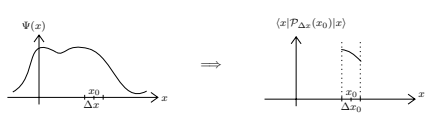
\includegraphics{immagini/19_image_2.png}
\end{center}
	
Le figure soprastanti mostrano cosa succede alla funzione d'onda. Prima della misura la funzione \'e nel suo stato iniziale $\Psi(x) = \braket{x}{\Psi}$ e ha come dominio tutto l'asse reale perch\'e la particella potr\'a trovarsi in qualsiasi punto; effettuando una misura ideale di prima specie il sistema \'e perturbato il meno possibile, per cui se la particella viene trovata all'interno dell'intervallo $\Delta x_0$, la funzione d'onda avr\'a la stessa forma precedente in quell'intervallo, mentre nella regione esterna collasser\'a a 0 (per cui dovr\'a essere rinormalizzata in accordo con l'interpretazione probabilistica di Born della funzione d'onda).
	

\begin{comment}
\subsubsection{Osservabili compatibili}
	
	Nel paragrafo precedente abbiamo considerato solamente osservabili a spettro non degenere, e abbiamo detto che immediatamente dopo la misura lo stato del sistema 'e completamente determinato perch´e 'e proiettato sull'autospazio relativo all'autovalore ak ∈ σd(A) trovato.
	
	Il caso non banale 'e quando ak 'e degenere, infatti dopo la misura possiamo solamente sapere che lo stato del sistema sta nell'autospazio multidimensionale relativo ad ak. Quindi per determinare univocamente lo stato 'e necessario misurare altre grandezze fisiche, con il requisito che non deteriorino l'informazione acquisita misurando A, ma anzi, la migliorino. Le osservabili per cui questo succede sono dette *osservabili compatibili* con A. Diamone la definizione operativa:
	Definizione 4. Immaginiamo che A e B siano grandezze fisiche a spettro discreto. Al tempo t *effettuiamo* una misura di A e otteniamo il risultato ak ∈ σd(A); subito dopo, cio'e prima che il sistema possa evolvere temporalmente in modo non banale, al tempo t
	+ facciamo una misura di B *ottenendo il risultato* bi ∈ σd(B),
	allora B 'e compatibile con A se ripetendo la misura di A *all'istante* t
	++ *otteniamo con certezza il valore* ak,
	∀ak, bi e ∀ *stato (cio'e non deve essere una particolare coincidenza).*
	Vediamo come tradurre nel linguaggio matematico della MQ questo risultato. Enunciamo e dimostriamo a tal proposito due teoremi.
	
	Teorema 1.3.1. A e B sono due osservabili compatibili ⇐⇒ *esiste una base ortonormale di autovettori comuni,*
	cio'e simultaneamente autovettori di A e B.
	
	Dimostrazione. =⇒: sappiamo che A e B essendo associati ad osservabili sono operatori autoaggiunti, allora qualsiasi vettore dello spazio di Hilbert pu'o essere decomposto in autostati dell'operatore A perch´e esiste sempre una base ortonormale di autovettori di questo operatore per H
	
	$$|\Psi\rangle=\sum_{a_{k}\in\sigma(A)}|\Psi_{a_{k}}\rangle$$
	
	in cui |\Psiak i 'e la proiezione del vettore sugli autospazi. Questo 'e ovviamente vero anche per l'operatore B
	
	$$|\Psi_{a_{k}}\rangle=\sum_{b_{i}\in\sigma(B)}|\Psi_{b_{i}}(a_{k})\rangle$$
	
	In generale se A e B sono operatori autoaggiunti qualsiasi, gli |\Psibi
	,(ak)i non rimangono pi'u autovettori dell'operatore A, questo per'o si verifica se A e B sono osservabili compatibili, quindi in questo caso sono loro autostati simultanei e li scriviamo come |\Psiak,bi i. Allora possiamo riscrivere il vettore come
	
	$\Psi\rangle=\sum_{a_{k}\in\sigma(A),b_{i}\in\sigma(B)}\Psi_{a_{k},b_{i}}\rangle\qquad\forall\,|\Psi\rangle\in\mathcal{H}$.  
	Se non c''e degenerazione, cio'e l'intersezione degli autospazi relativi ad ak e bi 'e unidimensionale, abbiamo concluso la dimostrazione; se invece c''e degenerazione, 'e sufficiente decomporre ogni autovettore all'interno degli autospazi di dimensione maggiore di 1 come |\PsiΦak,pi,τ i, e aggiungere una somma sull'indice τ che conta la degenerazione.
	
	⇐=: A e B possiedono una base di autovettori comuni |\Psiak,bi,τ i, allora il generico stato \Psi si pu'o decomporre in
	
	$$|\Psi\rangle=\sum_{a_{k},b_{i},\tau}c_{a_{k},b_{i},\tau}\left|\Psi_{a_{k},b_{i},\tau}\right\rangle$$
	
	Quello che fa la misura dell'osservabile A 'e eliminare la sommatoria sul suo spettro dato che 'e stato trovato solamente il valore ak, cio'e seleziona la proiezione ortogonale sull'autospazio relativo all'autovalore ak. Succede lo steso se effettuiamo la misura di B e otteniamo come risultato bi
	
	misura di $A\to\quad\sum_{b_{i},\tau}c_{a_{k},b_{i},\tau}\,|\,\Psi_{a_{k},b_{i},\tau}\rangle$ misura di $B\to\quad\sum_{\tau}c_{a_{k},b_{i},\tau}\,|\,\Psi_{a_{k},p_{i},\tau}\rangle$
	quindi resta solamente la somma sulla degenerazione residua. Ovviamente questi autovettori appartengono all'autospazio di A relativo all'autovalore ak, quindi effettuando una nuova misura di A non possiamo che trovare ak, e questa 'e esattamente la definizione che abbiamo dato per A e B osservabili compatibili.
	
	Un modo equivalente per enunciare questo risultato 'e di dire che se due osservabili sono compatibili possiamo decomporre l'intero spazio di Hilbert come la somma diretta degli autospazi relativi ai due operatori Hak,bi =
	Hak ∩ Hbi
	
	$$\mathcal{H}=\bigoplus_{a_{k}\in\sigma(A),b_{i}\in\sigma(B)}\mathcal{H}_{a_{k},b_{i}}$$
	$\texttt{1.3.2}$
	Inoltre questo teorema si pu'o estendere anche a operatori con spettro continuo, ricordando di considerare il problema agli autovalori generalizzato nello spazio delle distribuzioni, e di rimpiazzare le somme con gli integrali.
	
	Teorema 1.3.2. A e B sono due osservabili compatibili ⇐⇒ commutano tra loro, cio'e [*A, B*] = 0.
	
	Dimostrazione. =⇒: facciamo agire AB sul generico stato |\Psii e sfruttiamo il risultato del teorema precedente considerando una base di autovettori comuni di A e B
	
	$$AB\left|\Psi\right\rangle=AB\sum_{a_{k}\in\sigma(A),b_{i}\in\sigma(B)}\left|\Psi_{a_{k},b_{i}}\right\rangle=\sum_{a_{k},b_{i}}a_{k}b_{i}\left|\Psi_{a_{k},b_{i}}\right\rangle=\sum_{a_{k},b_{i}}b_{i}a_{k}\left|\Psi_{a_{k},b_{i}}\right\rangle$$ $$=A\sum_{a_{k},b_{i}}b_{i}\left|\Psi_{a_{k},b_{i}}\right\rangle=BA\sum_{a_{k},b_{i}}\left|\Psi_{a_{k},b_{i}}\right\rangle=BA\left|\Psi\right\rangle\quad\longrightarrow\quad[A,B]=0$$
	
	⇐=: dato che A 'e autoaggiunto possiamo decomporre lo spazio di Hilbert nella somma dei suoi autospazi H =Lak∈σ(A) Hak
	, quindi prendendo un qualsiasi vettore |\Psiak i ∈ Hak vale la seguente catena di uguaglianze
	
	$$A B\left|\Psi_{a_{k}}\right\rangle=B A\left|\Psi_{a_{k}}\right\rangle=B a_{k}\left|\Psi_{a_{k}}\right\rangle=a_{k}\big(B\left|\Psi_{a_{k}}\right\rangle\big)$$
	$$\square$$
	
	abbiamo ottenuto che B |\Psiak i 'e autostato di A relativo all'autovalore ak, cio'e Hak
	'e invariante sotto l'azione di B. Possiamo quindi considerare la restrizione di B che agisce su Hak e che rimane un operatore autoaggiunto:
	
	$$\mathcal{H}_{a_{k}}=\bigoplus_{b_{i}\in\sigma(B)}\mathcal{H}_{a_{k},b_{i}}\qquad\longrightarrow\qquad\mathcal{H}=\bigoplus_{a_{k}\in\sigma(A),b_{i}\in\sigma(B)}\mathcal{H}_{a_{k},b_{i}}$$
	
	Anche in questo caso il teorema si pu'o estendere facilmente al caso continuo con il consueto metodo.
	
	Se A e B sono limitati questo teorema 'e valido rigorosamente perch´e gli operatori possono essere definiti in tutto H, per cui D(A) = D(B) = D(AB) = D(BA). Per operatori illimitati ci possono essere casi patologici/particolari con problemi di dominio che non considereremo mai.
	
	Introduciamo ora un concetto molto importante per lo studio di un sistema quantistico: l'*insieme completo di* osservabili compatibili, chiamato pi'u semplicemente *ICOC*. La caratteristica di questo set di osservabili 'e che se effettuiamo una loro misura simultanea, identifichiamo il sistema in modo univoco, senza l'ambiguit'a che era presente nel caso dello spettro degenere.
	
	Definizione 5. *Consideriamo un vettore di N grandezze fisiche misurabili* A~ = (A1, ..., AN ) a cui associamo i rispettivi operatori A~ = (A1, A2, ..., AN ) *a spettro discreto. Supponiamo che queste osservabili siano compatibili* tra loro, e facciamo una misura di prima specie ottenendo come risultato il vettore ~a = (a1, ..., aN )*; sappiamo che* lo spazio HA = Ha1,...,aN sar'a dato dall'intersezione degli autospazi delle osservabili relativi ai diversi autovalori.
	
	Le osservabili saranno un ICOC se questo autospazio 'e non degenere, cio'e se ha dimensione unitaria.
	
	In generale, un insieme di osservabili deve verificare le seguenti due propriet'a per essere un ICOC: gli operatori commutano tra loro, e specificare un insieme di autovalori trovati con le misure determina univocamente lo stato del sistema. Quindi un modo equivalente per dire che un insieme di osservabili compatibili 'e completo 'e dire che esiste un'unica base ortonormale (a meno di fattori di fase) costituita tutta di autovettori simultanei di tutti gli operatori che costituiscono l'ICOC.
	
	Facciamo un esempio concreto. Per una particella priva di spin in una dimensione spaziale, X 'e un ICOC,
	perch´e sappiamo che esiste una base ortonormale generalizzata priva di degenerazione di oggetti del tipo ξx0
	(x) = δ(x−x0) per la quale 'e possibile scrivere qualsiasi stato del sistema. Allo stesso modo P 'e ICOC perch´e conoscere la decomposizione della trasformata di Fourier della funzione d'onda nello spazio delle P equivale ad avere l'informazione completa sullo stato del sistema. Si pu'o dimostrare che l'hamiltoniamo non 'e un ICOC,
	perch´e 'e quadratico nelle P, quindi per ogni valore di energia abbiamo una duplice degenerazione dello spettro delle onde piane, risulta quindi necessario un altro operatore, per esempio P, che ci permette di rimuovere tale degenerazione conoscendo il segno del momento.
	
	Avere un ICOC ci consente di dare una rappresentazione degli stati in termini di opportune funzioni d'onda.
	
	Prendiamo l'esempio precedente, H = L2(R) e X e P che sono due ICOC separatamente, con base generalizzata di vettori che soddisfano alle equazioni astratte in 1.4 Ogni elemento di H lo possiamo scrivere mediante le relazioni di completezza generalizzate per lo spettro continuo
	
	$$|\Psi\rangle=\int\mathrm{d}x\,|x\rangle\underbrace{\langle x|\Psi\rangle}_{\Psi(x)}\qquad\qquad|\Psi\rangle=\int\mathrm{d}p\,|p\rangle\underbrace{\langle p|\Psi\rangle}_{\Psi(p)}$$
	
	Pi'u in generale, possiamo applicare questo ragionamento a qualsiasi ICOC A~ con autovettori |~ai, i quali formano una base generalizzata per H, allora la decomposizione del ket |\Psii 'e del tutto analoga ai casi specifici precedenti
	
	$$|\Psi\rangle=\int\mathrm{d}\vec{a}\,|\vec{a}\rangle\underbrace{\langle\vec{a}|\Psi\rangle}_{\Psi(\vec{a})}$$
\end{comment}